% !TeX root = RJwrapper.tex
\title{Explaining Predictions with Shapley Values in R}
\author{by Brandon M. Greenwell and Christoph Molnar}

\maketitle

\abstract{%
An abstract of less than 150 words.
}

\hypertarget{warning}{%
\subsubsection{WARNING:}\label{warning}}

This article is very much a work in progress. Read at your own
risk\ldots{} If you notice a major issue, or have suggestions, feel free
to contribute!

\hypertarget{todo}{%
\subsubsection{TODO:}\label{todo}}

\begin{itemize}

  \item The notation is not consistent or fully explained (e.g., what is $x^\star$ in $f\left(x^\star\right) - \mathbb{E}\left[f\left(x\right)\right]$). Fix towards the end.

  \item \sout{Flesh out outline/section headers.}
  
  \item \sout{Finish bar tab example (or switch to something better).}
  
  \item Discuss SHAP as a unification of Shapley, LIME, etc.
  
  \item Find a good place to talk about "true to the model" versus "true to the data": https://arxiv.org/pdf/2006.16234.pdf (I think this is important for motivating the SampleSHAP approximation, which relies on randomly permuting instance values.) Some remarks on causality here are probably also warranted.
  
  \item Fill out KernelSHAP section.
  
  \item \sout{Find motivating example for **iml** package; maybe credit card default risk?}
  
  \item \sout{Find motivating example for **fastshap** package; maybe Ames housing?}
  
  \item \sout{Find motivating example of interfacing with **shap** via **reticulate**. Can probably lift from the **fastshap** vignette here: https://bgreenwell.github.io/fastshap/articles/fastshap-vs-shap.html.}
  
  \item Discuss advantages and disadvantages described in \url{https://christophm.github.io/interpretable-ml-book/shapley.html}.
  
  \item Mention the technical difference between SHAP (which satisfies the consistency property) and traditional Shapley values (like SampleSHAP), and how we loosen the distinction of the terminology here.
  
  \item Describe where the baseline ($\phi_0$) comes from, perhaps when introducing SHAP in the KernelSHAP section? Should make it clear that SampleSHAP also explains the difference $\widehat{f}\left(x\right) - \bar{y}_{trn}$, as opposed to $\widehat{f}\left(x\right)$ (not clear from reading \citet{strumbelj-2014-explaining}, maybe Equation (5)?).
  
  \item Is it worth mentioning the normal approximation discussed in \citet{strumbelj-2014-explaining}? (I honestly haven't seen this used anywhere, but that doesn't mean it's not valuable. Approximate standard errors? Confidence intervals? Need $\sigma_i ^ 2$.)
  
  \item Fix notation. $S$ is being used to represent the set of all players/features and subsets in some cases. Perhaps use $T \subseteq S$.
  
  \item Make it clear that Shapley values for machine learning help to explain $f\left(x^\star\right) - \mathbb{E}\left[f\left(x\right)\right]$, where $x^\star$ is a new observation and $\mathbb{E}\left[f\left(x\right)\right]$ is the baseline, or average training prediction.

\end{itemize}

\section{Background}

The \dfn{Shapley value} \citep{shapley-2016-value} is an idea from
coalitional/cooperative game theory. In a coalitional game, assume we
have \(p\) players that form a grand coalition (\(S\)) worth a certain
payout (\(\Delta_S\)). Suppose we also know how much any smaller
coalition (\(Q \subseteq S\)) (i.e., any subset of \(p\) players) is
worth (\(\Delta_Q\)). The goal is to distribute the total payout
\(\Delta_S\) to the individual \(p\) players in a ``fair'' way; that is,
so that each player receives their ``fair'' share. The Shapley value is
one such solution and the only one that uniquely satisfies a particular
set of ``fairness properties''.

Let \(v\) be a \dfn{characteristic function} that assigns a value to
each subset of players; in particular,
\(v : 2^p \rightarrow \mathbb{R}\), where \(v\left(S\right) = \Delta_S\)
and \(v\left(\emptyset\right) = 0\), where \(\emptyset\) is the empty
set (i.e., zero players). Let \(\phi_i\left(v\right)\) be the
contribution (or portion of the total payout) attributed to player \(i\)
in a particular game with total payout \(v\left(S\right) = \Delta_S\).
The Shapley value satisfies the following properties:

\begin{itemize}

  \item Efficiency: $\sum_{i = 1} ^ p \phi_i\left(v\right) = \Delta_S $.
  
  \item Null player: $\forall W \subseteq S \setminus \left\{i\right\}: \Delta_W = \Delta_{W \cup \left\{i\right\}} \implies \phi_i\left(v\right) = 0$.
  
  \item Symmetry: $\forall W \subseteq S \setminus \left\{i, j\right\}: \Delta_{W \cup \left\{i\right\}} = \Delta_{W \cup \left\{j\right\}} \implies \phi_i\left(v\right) = \phi_j\left(v\right)$.
  
  \item Linearity: If $v$ and $w$ are functions describing two coalitional games, then $\phi_i\left(v + w\right) = \phi_i\left(v\right) + \phi_i\left(w\right)$.

\end{itemize}

The above properties can be interpreted as follows: 1) the individual
player contributions sum to the total payout, hence, are implicitly
normalized; 2) if a player does not contribute to the coalition they
receive a payout of zero; 3) if two players have the same impact across
all coalitions, they receive equal payout; and 4) the local
contributions are additive across different games.

\citep{shapley-2016-value} showed that the unique solution satisfying
the above properties is given by

\begin{equation}
\label{eqn:shapley-value}
\phi_i\left(x\right) = \frac{1}{p!} \sum_{\mathcal{O} \in \pi\left(p\right)} \left[v\left(S^\mathcal{O} \cup i\right) - v\left(S^\mathcal{O}\right)\right], \quad i = 1, 2, \dots, p,
\end{equation} where \(\mathcal{O}\) is a specific permutation of the
players indices \(\left\{1, 2, \dots, p\right\}\), \(\pi\left(p\right)\)
is the set of all such permutations of size \(p\), and \(S^\mathcal{O}\)
is the set of players joining the coalition before player \(i\).

In other words, the Shapley value is the average marginal contribution
of a player across all possible coalitions in a game. Another way to
interpret Equation \eqref{eqn:shapley-value} is as follows. Imagine the
coalitions (subsets of players) being formed one player at a time (which
can happen in different orders), with the \(i\)-th player demanding a
fair contribution/payout of
\(v\left(S^\mathcal{O} \cup i\right) - v\left(S^\mathcal{O}\right)\).
The Shapley value for player \(i\) is given by the average of this
contribution over all possible permutations in which the coalition can
be formed.

A simple example may help clarify the main ideas. Suppose three friends
(players)---Alex, Brad, and Brandon---decide to go out for drinks after
work (the game). They shared a few pitchers of beer, but nobody payed
attention to how much each person drank (collaborated). What's a fair
way to split the tab (total payout)? Suppose we knew the follow
information, perhaps based on historical data:

\begin{itemize}

  \item If Alex drank alone, he'd only pay \$10.
  
  \item If Brad drank alone, he'd only pay \$20.
  
  \item If Brandon drank alone, he'd only pay \$10.
  
  \item If Alex and Brad drank together, they'd only pay \$25.
  
  \item If Alex and Brandon drank together, they'd only pay \$15.
  
  \item If Brad and Brandon drank together, they'd only pay \$13.
  
  \item If Alex, Brad, and Brandon drank together, they'd only pay \$30.

\end{itemize}

With only three players, we can enumerate all possible coalitions. In
Table \ref{tab:bar}, we list out all possible permutations of the three
players and list the marginal contribution of each. Take the first row,
for example. In this particular permutation, we start with Alex. We know
that if Alex drinks alone, he'd spend \(10\), so his marginal
contribution by entering first is \(10\). Next, we assume Brad enters
the coalition. We know that if Alex and Brad drank together, they'd pay
a total of \(25\), leaving \(15\) left over for Brad's marginal
contribution. Similarly, if Brandon joins the party last, his marginal
contribution would be only \(5\) (the difference between \(30\) and
\(25\)). The Shapley value for each player is the average across all six
possible permutations (these are the column averages reported in the
last row). In this case, Brandon would get away with the smallest payout
(i.e., have to pay the smallest portion of the total tab). The next time
the bartender asks how you want to split the tab, whip out a pencil and
do the math!

\textbf{FIXME:} Connect some of the values in this example with Equation
\ref{eqn:shapley-value} (e.g., show what
\(v\left(S^\mathcal{O} \cup i\right)\) is in this example).

\begin{table}[!htb]
\centering
\begin{tabular}{@{}llll@{}}
\toprule
                      & \multicolumn{3}{l}{Marginal contribution} \\ \midrule
Permutation/order of players           & Alex        & Brad         & Brandon      \\ \midrule
Alex, Brad, Brandon   & \$10        & \$15         & \$5          \\ 
Alex, Brandon, Brad   & \$10        & \$15         & \$5          \\
Brad, Alex, Brandon   & \$5         & \$20         & \$5          \\
Brad, Brandon, Alex   & \$10        & \$20         & \$0          \\
Brandon, Alex, Brad   & \$5         & \$15         & \$10         \\
Brandon, Brad, Alex   & \$17        & \$3          & \$10         \\ \midrule
Shapley contribution: & \$9.50      & \$14.67      & \$5.83       \\ \bottomrule
\end{tabular}
\caption{Marginal contribution for each permutation of the players \{Alex, Brad, Brandon\} (i.e., the order in which they arrive). The Shapley contribution is the average marginal contribution across all permutations. (Notice how each row sums to the total bill of \$30.) \label{tab:bar}}
\end{table}

\subsection{Shapley values for explaining predictions}

\citet{strumbelj-2014-explaining} suggested using the Shapley value
(Equation \eqref{eqn:shapley-value}) to help explain predictions from a
machine learning model. In the context of statistical/machines learning,

\begin{itemize}

  \item A game is represented by the prediction task for a single observation $x$.
  
  \item The total payout/worth ($\Delta_S$) for $x$ is the prediction for $x$ minus the average prediction for all training observations (call this the baseline prediction).
  
  \item The players are the individual feature values of $x$ that collaborate to receive the payout (i.e., predict a certain value).
  
\end{itemize}

In the following sections, we'll discuss several popular ways to compute
Shapley values in practice.

\textbf{FIXME:} Make it clear that Shapley values help explain
\(f\left(x^\star\right) - \mathbb{E}\left[f\left(x\right)\right]\), not
\(f\left(x^\star\right)\) directly. Also mention that Shapley values can
be used to decompose model loss/accuracy (e.g., logloss or \(R^2\)).

\subsection{Choice of characteristic function $v$}

\textbf{FIXME:} Need to make it clear how \(v\left(S\right)\) is
computed in the context of a machine learning model; maybe come up with
a numeric example?

\textbf{FIXME:} Clear up notation (e.g., \(S^c\) or \(x_{S^c}\)?)

The challenge of using Shapley values for the purpose of explaining
predictions is in defining the functional form of \(v\). As discussed in
\citet{chen-2020-true}, there are several ways to do this. However,
since we are primarily interested in understanding how much each feature
contributed to a particular prediction, \(v\) is typically related to a
conditional expectation of the model's prediction.
\citet{chen-2020-true} make the distinction between two possibilities,
each of which differs in their conditioning argument. The Shapley value
implementations discussed in this paper (e.g., KernelSHAP and TreeSHAP)
rely on what \citet{chen-2020-true} call the
\dfn{interventional conditional expectation}, which can be expressed
using \citeauthor{pearl-2009-causality}'s
\citeyearpar{pearl-2009-causality} \(do\left(\cdot\right)\) operator:
\begin{equation}
\label{eqn:ice}
\begin{split}
  v\left(S\right) &= \mathbb{E}\left[f\left(x_S, x_{S^c}\right) | do\left(x_S\right)\right] \\
                  &= \int f\left(x_S, x_{S^c}\right) p\left(x_{S^c}\right) d x_{S^c},
\end{split}
\end{equation} where \(S^c\) is the complement \(S\), \(x_S\) and
\(x_{S^c}\) are the set of features in \(S\) and \(S^c\), respectively,
and \(p\left(x_{S^c}\right)\) is the joint probability density of
\(x_{S^c}\). Equation \eqref{eqn:ice} can be interpreted as the expected
value of \(f\left(x\right)\) given some intervention on the features in
\(S\), which assumes independence between \(x_S\) and \(x_{S^c}\); a
similar assumption is also used in the construction of
\dfn{partial dependence plots} \citep{friedman-2001-greedy}, with the
connection to \citeauthor{pearl-2009-causality}'s
\citeyearpar{pearl-2009-causality} \(do\left(\cdot\right)\) operator
established in \citet{zhao-2021-causal}. Shapley values based on this
formulation of \(v\) are referred to as
\dfn{interventional Shapley values} \citep{chen-2020-true}. The various
Shapley value algorithms discussed over the next several sections fall
under this form.

\textbf{FIXME:} Connect to other permute-and-predict methods advocated
against in Hooker (2019)? Source:
\url{https://arxiv.org/pdf/1905.03151.pdf}.

\section{Estimating Shapley values/feature contributions in practice}

In this section, we'll detail several algorithms for estimating Shapley
values for the purpose of explain predictions from a machine learning
model.

\subsection{SampleSHAP: Approximate Shapley values via Monte Carlo simulation \label{sec:SampleSHAP}}

Computing the exact Shapley value is computationally infeasible, even
for moderately large \(p\). To that end,
\citet{strumbelj-2014-explaining} suggest a Monte Carlo approximation,
which we'll call
SampleSHAP\^{}\footnote{**FIXME:** Make a note on the technical use of the term SHAP, and how we're being loose with the terminology here.},
that assumes independent
features\footnote{While SampleSHAP, along with many other common Shapley value procedures, assumes independent features, several arguments can be made in favor of this assumption; see, for example, \citet{chen-2020-true} and the references therein.}.
Their approach is described in Algorithm \ref{alg:SampleSHAP}.

Here, A single estimate of the contribution of \(x_i\) to
\(f\left(x^\star\right) - \mathbb{E}\left[f\left(x\right)\right]\) is
nothing the more than the difference between two predictions, where each
prediction is based on a set of ``Frankenstein
instances''\^{}\footnote{The terminology used here takes inspiration from \citet[p. 231]{molnar-2019-iml}.}
that are constructed by swapping out values between the instance being
explained (\(x\)) and an instance selected at random from the training
data. To help stabilize the results, the procedure is repeated a large
number, say, \(R\), times, and the results averaged together.

\begin{algorithm}
\begin{enumerate}
  \item For $j = 1, 2, \dots, R$:
  \begin{enumerate}
    \item Select a random permutation $\mathcal{O}$ of the sequence $1, 2, \dots, p$.
    \item Select a random instance $w$ from the set of training observations $\boldsymbol{X}$.
    \item Construct two new instances as follows:
    \begin{itemize}
      \item $b_1 = x$, but all the features in $\mathcal{O}$ that appear after feature $x_i$ get their values swapped with the corresponding values in $w$.
      \item $b_2 = x$, but feature $x_j$, as well as all the features in $\mathcal{O}$ that appear after $x_j$, get their values swapped with the corresponding values in $w$.
    \end{itemize}
    \item $\phi_{ij}\left(x\right) = f\left(b_1\right) - f\left(b_2\right)$.
  \end{enumerate}
  \item $\phi_i\left(x\right) = \sum_{j = 1} ^ R \phi_{ij}\left(x\right) / R$.
\end{enumerate}
\caption{Approximating the $i$-th feature's contribution to $f\left(x\right)$. \label{alg:SampleSHAP}}
\end{algorithm}

If there are \(p\) features and \(m\) instanced to be explained, this
requires \(2 \times R \times p \times m\) predictions (or calls to a
scoring function). In practice, this can be quite computationally
demanding, especially since \(R\) needs to be large enough to produce
good approximations to each \(\phi_i\left(x\right)\). How large does
\(R\) need to be to produce accurate explanations? It depends on the
variance of each feature in the observed training data, but typically
\(R \in \left[30, 100\right]\) will suffice (\textbf{FIXME:} Is there a
good reference for this?). In Section \ref{sec:fastshap}, we'll discuss
a particularly optimized implementation of Algorithm
\ref{alg:SampleSHAP} that only requires \(2mp\) calls to a scoring
function.

SampleSHAP can be computationally prohibitive if you need to explain
large data sets. Fortunately, you often only need to explain a handful
of predictions, for example the most extreme predictions. However,
generating explanations for the entire training set, or a large enough
sample thereof, can be useful for generating aggregated model summaries,
like Shapley-based variable importance plots \textbf{FIXME:} Add
reference.

\subsection{LinearSHAP: Shapley values from additive linear models \label{sec:LinearSHAP}}

\textbf{FIXME:} Proof of the following is given in
\citet{aas-2020-explaining}.

First, lets discuss how a feature's value contributes to a prediction
\(f\left(X\right)\) in a simple (additive) linear model with independent
features. That is, let's assume for a moment that \(f\) takes the form
\begin{equation}
\nonumber
  f\left(X\right) = \beta_0 + \beta_1 X_1 + \dots + \beta_p X_p
\end{equation}

Recall that the contribution of the \(i\)-th feature to the prediction
\(f\left(X\right)\) is the difference between \(f\left(X\right)\) and
the expected prediction if the \(i\)-th feature's value were not known:
\begin{equation}
\nonumber
\begin{split}
  \phi_i\left(X\right) &= \beta_0 + \dots + \beta_i X_i + \dots + \beta_p X_p \\ &\quad\quad - \left(\beta_0 + \dots + \beta_i \E\left(X_i\right) + \dots + \beta_p X_p\right) \\
  &= \beta_i \left(X_i - \E\left(X_i\right)\right)
\end{split},
\end{equation} where we estimate \(\E\left(X_i\right)\) with the
corresponding sample mean \(\bar{X}_i\). The quantity
\(\phi_i\left(X\right)\) is also referred to as the
\emph{situational importance of $X_i$} \citep{achen-1982-interpreting}.

Note that if you're using R, then
\(\beta_i \left(X_i - \E\left(X_i\right)\right)\) is exactly what's
returned by R's \code{predict()} method when applied to \code{lm/glm}
models, provided you specify \code{type = "terms"}; see
\code{?predict.lm} for details and Section \ref{sec:benchmark} for an
example with a logistic regression model.

\subsection{KernelSHAP: Approximate Shapley values using kernel approximations}

\textbf{NOTES:}

(Christoph, this was my initial ``thought dump'', feel free to delete or
use.)

\begin{itemize}

  \item Discuss SHAP (Shapley Additive Explanations).

  \item The KernelSHAP supposedly requires less computational power than SampleSHAP to obtain a similar approximation accuracy (i.e., fewer replications).

  \item KernelSHAP, or at least it's implementation in \pkg{shap}, distributes the number of replications unevenly across the different features. Apparently, features with higher variance are attributed more replications. 

  \item Like SampleSHAP and LinearSHAP, KernelSHAP assumes independent features.

  \item Extended to handle dependent features in \citet{aas-2020-explaining} and is available in the R package \CRANpkg{shapr} \citep{R-shapr}. 

  \item KernelSHAP \citep{lundberg-2017-KernelSHAP} uses a specially-weighted local linear regression to estimate SHAP values for any model. Unlike SampleSHAP...

  \item SHAP decomposes a prediction into 
\begin{equation}
\label{eqn:shap}
  f\left(x\right) = \phi_0 + \sum_{i = 1} ^ p \phi_i,
\end{equation}
where $f\left(x\right)$, $\phi_0 = \mathbb{E}\left[f\left(x\right)\right]$, $p$ is the number of predictors, and $\phi_i$ is the contribution of the $i$-th feature. It should be noted that $\phi_i$ ($i = 1, 2, \dots, p$) depend on the observation $x$, whereas $\phi_0$ is constant. From Equation \eqref{eqn:shap}, it should be clear that $\sum_{i = 1}^p \phi_i = f\left(x\right) - \phi_0$. In other words, SHAP values help to explain the difference between a particular prediction and the global average prediction. The quantity $\phi_0$ is often referred to as the baseline prediction and is estimated in practice using the average prediction across all $N$ training observations: $\bar{y}_{trn} = \sum_{i = 1}^N y_i / N$

  \item \citet{covert-2021-improving} (and the corresponding GitHub repo: \url{https://github.com/iancovert/shapley-regression}) offer a nice discussion on KernelSHAP and some insight into its properties.

  \item Discuss Shapley values as the solution to a weighted least squares problem; see \citet{charnes-1988-extremal} for details.

\end{itemize}

\subsection{TreeSHAP: Efficient Shapley values for tree ensembles}

\textbf{FIXME:} Need to find the right balance of details and complexity
here.

\textbf{NOTES:}

TreeSHAP assumes ``less'' feature independence in the sense that it
accounts for some of the dependence, but not all
\citep{aas-2020-explaining}.

Only applicable to tree-based models, and implemented for only a few
algorithms (e.g., XGBoost and LightGBM).

\section{Shapley values is R (and other open source software)}

\textbf{TODO:} Use \pkg{pkgsearch} to do a more exhaustive check. Also,
reference the landscape paper:
\url{https://arxiv.org/pdf/2009.13248.pdf}.

Probably the first, and most widely used implementation of Shapley
explanations is the Python \pkg{shap} library
\citep{lundberg-2017-KernelSHAP}, which provides a Python implementation
of SampleSHAP, KernelSHAP, TreeSHAP, and a few other model-specific
Shapley methods (e.g., DeepSHAP, which is provides approximate Shapley
values for deep learning models).

The \CRANpkg{iml} package \citep{R-iml} provides the \code{Shapley()}
function, which is a direct implementation of Algorithm
\ref{alg:SampleSHAP}. It is written in \CRANpkg{R6} \citep{R-R6}.

Package \CRANpkg{iBreakDown} implements a general approach to explaining
the predictions from supervised models, called \dfn{Break Down}
\citep{gosiewska-2019-iBreakDown}. SampleSHAP values can be computed as
a special case from random Break Down profiles; see
\code{iBreakDown::\code{shap()} for details}.

\CRANpkg{shapper} provides an R interface to the Python \pkg{shap}
library using \CRANpkg{reticulate} \citep{R-reticulate}; however, it
currently only supports KernelSHAP (\pkg{shap} itself supports
SampleSHAP, TreeSHAP, LinearSHAP, as well as various other
model-specific Shapley explanation methods).

\textbf{FIXME:} \pkg{shapr} is now on CRAN!

We're also aware of two experimental packages supporting Shapley
explanations that are not currently on CRAN: \pkg{shapr}
\citep{R-sellereite} and \pkg{shapFlex} \citep{R-shapFlex}. As
previously discussed, one drawback of traditional Shapley values is the
assumption of independent features (an assumption made by many IML
procedures, in fact). To that end, the \pkg{shapr} package implements
Shapley explanations that can account for the dependence between
features \citep{aas-2019-explaining}, resulting in significantly more
accurate approximations to the Shapley values. The package also includes
an implementation of KernelSHAP that's consistent with the \pkg{shap}
package for Python. The \pkg{shapFlex} package, short for Shapley
flexibility, provides approximate Shapley values that incorporate causal
constraints into the model's feature space, as described in
\citet{frye-2019-asymmetric}.

TreeSHAP has been directly incorporated into most implementations of
XGBoost \citep{chen-2016-xgboost} (including \CRANpkg{xgboost}
\citep{R-xgboost}), CatBoost \citep{eronika-2017-catboost}, and LightGBM
\citep{ke-2017-lightgbm}. Both \CRANpkg{fastshap} \citep{R-fastshap} and
\CRANpkg{SHAPforxgboost} \citep{R-SHAPforxgboost} provide an interface
to \pkg{xgboost}'s TreeSHAP implementation.

\CRANpkg{fastshap} provides an efficient implementation of SampleSHAP
and makes it a viable option for explaining the predictions from model's
where efficient model-specific Shapley methods do not exist or are not
yet implemented.

In Julia, there's \pkg{SampleSHAP.jl}, which is a lightweight port of
\pkg{fastshap}; \pkg{ShapML.jl}, which is another Julia implementation
of SampleSHAP; and \pkg{ShapleyValues.jl}, which hasn't been updated
since 2016.

The next two sections illustrate more in-depth use of the \pkg{iml} and
\pkg{fastshap} packages, respectively.

\subsection{The \pkg{iml} package}

The \pkg{iml} package includes a consistent interface to several machine
learning interpretability methods, including: variable importance plots,
as described in \citet{fisher-2019-models}, accumulated local effects
(ALE) plots \citep{apley-2019-ale}; partial dependence plots
\citep{friedman-2001-greedy}, individual conditional expectation (ICE)
curves \citep{goldstein-peeking-2015}, the SampleSHAP algorithm
described in \citet{strumbelj-2014-explaining} and discussed in Section
\ref{sec:SampleSHAP}, the \(H\)-statistic for quantifying the strength
of interaction effects \citep{friedman-2008-predictive}, tree-based
surrogate models (see, for example, \citet[Chap. 5]{molnar-2019-iml}),
and others.

The \code{iml::Shapley()} function implements the SampleSHAP
approximation described in Section \ref{sec:SampleSHAP}.

\subsubsection{Example: credit card default}

To illustrate the use of \code{iml::Shapley()} we'll use the credit card
default data set \citep{cheng-2009-credit} available from the UCI
Machine Learning Repository at
\url{https://archive.ics.uci.edu/ml/datasets/default+of+credit+card+clients#}.

To start, we'll download the data set into a file named
\file{credit.xls}. Since it's an Excel file, we can read the data into R
using the \CRANpkg{readxl} package \citep{R-readxl}:

\begin{Schunk}
\begin{Sinput}
# Download and read in the credit default data from the UCI ML repo
tf <- tempfile(fileext = ".xls")
url <- paste0("https://archive.ics.uci.edu/ml/machine-learning-databases/",
              "00350/default%20of%20credit%20card%20clients.xls")
download.file(url, destfile = tf)
credit <- as.data.frame(readxl::read_xls(tf, skip = 1))
\end{Sinput}
\end{Schunk}

Next, we'll clean up the data set a bit by fixing the column names,
re-encoding some of the categorical variables, removing the ID column,
and coercing categorical variables to factors. A detailed description of
the columns can be found in \citep{cheng-2009-credit}, or at
\url{https://archive.ics.uci.edu/ml/datasets/default+of+credit+card+clients#}

\begin{Schunk}
\begin{Sinput}
# Clean up column names a bit
names(credit) <- tolower(names(credit))
names(credit)[names(credit) == "default payment next month"] <- "default"
credit$id <- NULL  # remove ID column

# Clean up categorical features
credit$sex <- ifelse(credit$sex == 1, yes = "male", no = "female")
credit$education <- ifelse(
  test = credit$education == 1, 
  yes = "graduate school", 
  no = ifelse(
    test = credit$education == 2, 
    yes = "university",
    no = ifelse(
      test = credit$education == 3,
      yes = "high school",
      no = "other"
    )
  )
)
credit$marriage <- ifelse(
  test = credit$marriage == 1, 
  yes = "married",
  no = ifelse (
    test = credit$marriage == 2,
    yes = "single",
    no = "other"
  )
)
credit$default <- ifelse(credit$default == 1, yes = "yes", no = "no")

# Coerce to factors
for (i in seq_len(ncol(credit))) {
  if (is.character(credit[[i]])) {
    credit[[i]] <- as.factor(credit[[i]])
  }
}
\end{Sinput}
\end{Schunk}

Finally, we'll split the data into train test/test sets using a 70/30
split:

\begin{Schunk}
\begin{Sinput}
set.seed(1342)  # for reproducibility
ids <- sample(nrow(credit), size = 0.7 * nrow(credit), replace = FALSE)
credit.trn <- credit[ids, ]  # train
credit.tst <- credit[-ids, ]  # test
head(credit.trn)
\end{Sinput}
\begin{Soutput}
#>       limit_bal    sex       education marriage age pay_0 pay_2 pay_3 pay_4
#> 8320      5e+04   male      university  married  42     0     0     0     0
#> 27602     2e+04 female      university   single  27     0     0     0     0
#> 16068     8e+04 female      university   single  31     0     0     2     2
#> 4729      5e+04 female graduate school   single  26     0     0     2     2
#> 4241      2e+05   male graduate school  married  34    -1    -1    -1    -1
#> 10363     6e+04 female     high school   single  40     0     0     0     0
#>       pay_5 pay_6 bill_amt1 bill_amt2 bill_amt3 bill_amt4 bill_amt5 bill_amt6
#> 8320      0    -1     46100     46949     18755     11112     11374      5919
#> 27602     0    -1     18854     19116     15030     13025     12223     15975
#> 16068     0     0     75953     81055     81587     78103     78335     78678
#> 4729      2     2      5800      8189      7909      9767      9466     11300
#> 4241     -1    -2      5879      5884      5171      4598       -95     -2175
#> 10363     0     0     35602     35911     36246     29831     29667     30062
#>       pay_amt1 pay_amt2 pay_amt3 pay_amt4 pay_amt5 pay_amt6 default
#> 8320      2133     1058     2000     2043     5919    16346     yes
#> 27602     1292     1509     1522     3111    20000     1121      no
#> 16068     7000     3000        0     3000     3100     5900      no
#> 4729      2500        0     2000        0     2000      400     yes
#> 4241      5884     5171     4598        0        0        0      no
#> 10363     1654     1762     1044     1065     1266      979      no
\end{Soutput}
\end{Schunk}

For modeling, we'll fig a gradient boosted tree ensemble (GBM) using the
\CRANpkg{R-gbm} package (originally by Greg Ridgeway). While more
efficient and scalable GBM implementations certainly exist in R (e.g.,
\pkg{xgboost} and \pkg{lightgbm}), they don't often support categorical
features without having to re-encode them numerically.

\begin{Schunk}
\begin{Sinput}
library(gbm)

# gbm required the target to be coded as 0/1
credit.trn$default <- ifelse(credit.trn$default == "yes", 1, 0)

# Fit a GBM to the credit default training set
set.seed(1554)  # for reproducibility
bst <- gbm(default ~ ., data = credit.trn, distribution = "bernoulli", 
           n.trees = 300, interaction.depth = 5, shrinkage = 0.1, cv.folds = 5)

# Plot results and print optimal number of trees
par(las = 1)  # horizontal y-axis labels
(best <- gbm.perf(bst, plot.it = TRUE, method = "cv"))
\end{Sinput}
\begin{figure}[!htb]

{\centering 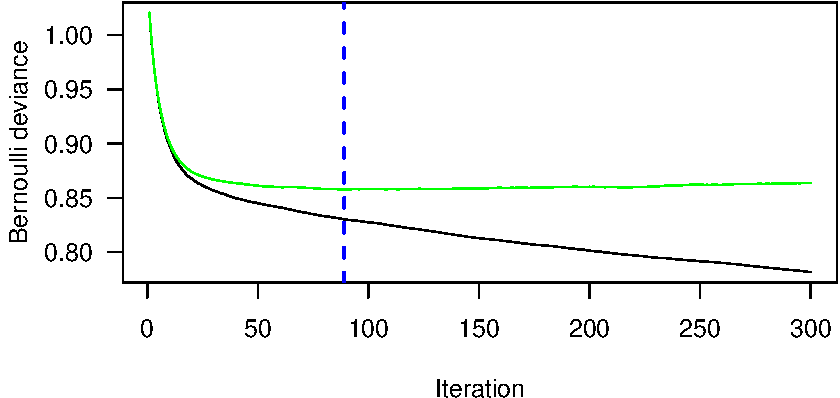
\includegraphics[width=1\linewidth]{greenwell_files/figure-latex/ex-credit-gbm-1} 

}

\caption[5-fold cross-validation performance as a function of the number of trees from the GBM model applied to the credit default data set]{5-fold cross-validation performance as a function of the number of trees from the GBM model applied to the credit default data set.}\label{fig:ex-credit-gbm}
\end{figure}
\begin{Soutput}
#> [1] 89
\end{Soutput}
\end{Schunk}

To use the \pkg{iml} package with out \pkg{gbm} model, we need to create
a \code{Predictor} object; that is, a special object used by the
functions in the \pkg{iml} package that holds the fitted machine
learning model as well as any required metadata (e.g., the training data
and a prediction wrapper so that \pkg{iml} knows how to obtain new
predictions from your model). Below we construct a \code{Predictor}
object for the previously fit \pkg{gbm} model. (Note that the prediction
wrapper, \code{pfun()}, returns predictions on the logit scale.)

\begin{Schunk}
\begin{Sinput}
# Prediction wrapper
pfun <- function(object, newdata) {
  predict(object, newdata = newdata, n.trees = best)
}

# Construct a `Predictor` object
predictor <- iml::Predictor$new(bst, data = credit.trn, y = "default",
                                predict.fun = pfun)
\end{Sinput}
\end{Schunk}

We can now compute Shapley values for any observation (e.g., instances
from the training set or a new instance). Here, we'll compute the
feature contributions for the most extreme prediction in the test set.
In this case, the maximum prediction (on the logit scale) is
\texttt{2.639} corresponds to an estimated probability of roughly
\texttt{0.933}.

\begin{Schunk}
\begin{Sinput}
# Compute test set predictions
max(p <- pfun(bst, newdata = credit.tst))
\end{Sinput}
\begin{Soutput}
#> [1] 2.638971
\end{Soutput}
\begin{Sinput}
# Compute approximate Shapley values for the most extreme prediction
set.seed(2241)  # for reproducibility
(ex <- iml::Shapley$new(predictor, x.interest = credit.tst[which.max(p), ], 
                        sample.size = 100))
\end{Sinput}
\begin{Soutput}
#> Interpretation method:  Shapley 
#> Predicted value: 2.638971, Average prediction: -1.497362 (diff = 4.136333)
#> 
#> Analysed predictor: 
#> Prediction task: unknown 
#> 
#> 
#> Analysed data:
#> Sampling from data.frame with 21000 rows and 23 columns.
#> 
#> Head of results:
#>     feature         phi     phi.var        feature.value
#> 1 limit_bal -0.16780381 0.073059029     limit_bal=340000
#> 2       sex -0.01610681 0.001496965           sex=female
#> 3 education  0.08189806 0.045681690 education=university
#> 4  marriage -0.04323803 0.007992601      marriage=single
#> 5       age -0.04727680 0.003910510               age=31
#> 6     pay_0  1.25911873 0.500260821              pay_0=5
\end{Soutput}
\end{Schunk}

The output provides lots of relevant information. The predicted value
for this observation is roughly 2.639 (on the logit scale), which is
nearly 4.136 more than the baseline or average training prediction of
-1.497. We can also see the explanations for the first few features. The
approximate Shapley values, based on \(R = 100\) replications of
Algorithm \ref{alg:SampleSHAP}, are given in the column labeled
\code{phi}. The corresponding sample variance of each is given in column
\code{phi.var}. In this example, we can see that \code{pay\_0=5}
contributed roughly 1.259 to the 4.136 difference.

It can often be useful to plot the feature contributions from a single
explanation. With \pkg{iml}, you can just call the \code{plot()} method
on the Shapley output:

\begin{Schunk}
\begin{Sinput}
# Plot feature contributions
plot(ex)  # Figure XYZ
\end{Sinput}
\begin{figure}[!htb]

{\centering 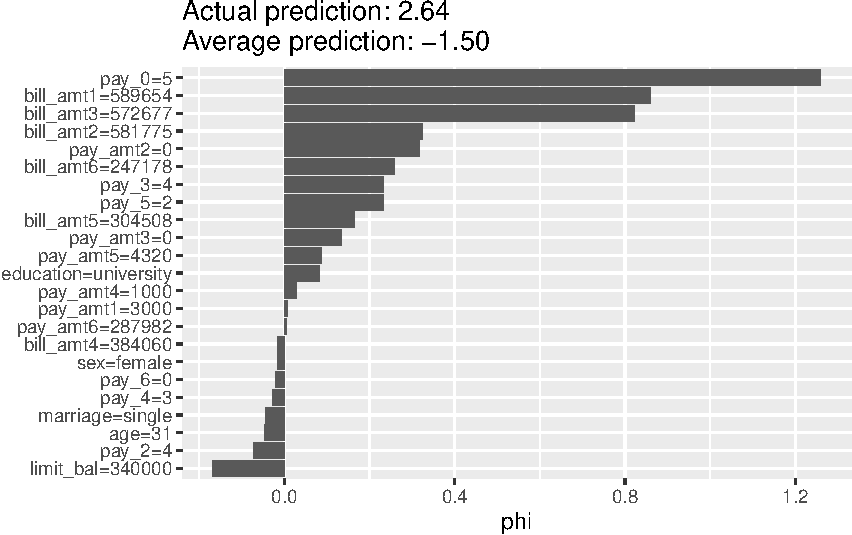
\includegraphics[width=1\linewidth]{greenwell_files/figure-latex/ex-credit-gbm-predict-extreme-explain-plot-1} 

}

\caption[Approximate Shapley contributions for the most extreme prediction in the test set for the credit card default example]{Approximate Shapley contributions for the most extreme prediction in the test set for the credit card default example. The predicted value for this observation is roughly 2.64 (on the logit scale), which is nearly 4.14 more than the baseline or average training prediction of -1.50. The three biggest contributers to this difference are \code{pay\_0}, \code{bill\_amt1}, and \code{bill\_amt3}, each of which had a positive contribution to the difference.}\label{fig:ex-credit-gbm-predict-extreme-explain-plot}
\end{figure}
\end{Schunk}

\subsection{The \pkg{fastshap} package \label{sec:fastshap}}

Like many post-hoc interpretation techniques (e.g., PDPs and ICE
curves), SampleSHAP can be made more efficient by generating all the
data up front, and scoring it only once (or twice, in the case of
SampleSHAP). For example, PDPs and ICE curves can be efficiently
constructed with only a single call to a scoring function by generating
all of the required data up front using a single cross-join operation
(which can be done rather efficiently in SQL or Spark). The scored data
can then be post-processed/aggregated and displayed as either a PDP or
set of ICE curves. An example using Spark with \CRANpkg{sparklyr}
\citet{R-sparklyr} can be found here:
\url{https://github.com/bgreenwell/pdp/issues/97}.

Fortunately, a similar trick can be exploited for SampleSHAP. Whether
explaining a single instance using a large number of Monte Carlo
repetitions (\(R\)), or explaining a large number of instances with with
\(R = 1\), the basic idea is to generate all the required Frankenstein
instances (Section \ref{sec:SampleSHAP}) \(b_1\) and \(b_2\) upfront,
and stored in matrices \(\boldsymbol{B}_1\) and \(\boldsymbol{B}_2\),
respectively.

For example, suppose we wanted to estimate the contribution of \(x_i\)
for each of the \(N\) rows of the available training data
\(\boldsymbol{X}\) using a single Monte-Carlo repetition in Algorithm
\ref{alg:SampleSHAP} (i.e.,
\(R = 1\))\footnote{The same idea also extends to explaining new instances.}.
To start, we can generate the \(N\) random instances at once and store
them in an \(N \times p\) matrix \(\boldsymbol{W}\). Rather generating
\(N\) random permutations \(\mathcal{O}\), and constructing \(b_1\) and
\(b_2\) one at a time, the \pkg{fastshap} package uses C++---via
\CRANpkg{Rcpp} \citep{R-Rcpp}---to efficiently generate an
\(N \times p\) logical matrix \(\boldsymbol{\mathcal{O}}\), where
\(\boldsymbol{\mathcal{O}}_{kl} = 1\) if feature \(x_l\) appears before
feature \(x_i\) in the \(k\)-th permutation, and \(0\) otherwise. This
logical matrix can then be used to logically subset \(\boldsymbol{X}\)
and \(\boldsymbol{W}\) to more efficiently construct
\(\boldsymbol{B}_1\) and \(\boldsymbol{B}_2\) in a single swoop. The
matrices (or data frames) can then be each scored once, and the
difference taken, to generate a single replication of
\(\phi_i\left(x\right)\) for each row of \(\boldsymbol{X}\).

Suppose instead we want to estimate the contribution of \(x_i\) for a
single instance \(x\), but using a large value of \(R\) for accuracy. We
could employ the same trick, but in this case \(\boldsymbol{X}\) would
refer to the \(R \times p\) matrix, where each row is a copy of the
instance \(x\).

\pkg{fastshap} also uses efficient exact methods for the special cases
described in Sections\ldots{}

\pkg{fastshap} is faster at computing Shapley values for a single
feature for a large number of instances (or a large value of \(R\) for a
single instance). But what about a large number of features?
Fortunately, Algorithm \ref{alg:SampleSHAP} can be trivially
parallelized across features, and this is built into \pkg{fastshap}.

\subsubsection{Example: Ames housing data}

\textbf{FIXME:} Rerun with \texttt{exact\ =\ TRUE} and show how total
across each is equal to the difference between prediction and baseline.

For illustration, we'll use the Ames housing data \citep{ames-cock-2011}
which are available in the \CRANpkg{AmesHousing} package
\citep{R-AmesHousing}. These data describe the sale of individual
residential properties in Ames, Iowa from 2006--2010. The data set
contains 2930 observations, 80 features (23 nominal, 23 ordinal, 14
discrete, and 20 continuous), and a continuous target giving the sale
price of the home (\code{Sale\_Price}). The version we'll load is a
cleaned up version of the original data set and treats all categorical
variables as nominal (see \code{?AmesHousing::make\_ames} for details).

To start, we'll load the Ames housing data from the
\CRANpkg{AmesHousing} package \citep{R-AmesHousing} and fit a (default)
random forest to the entire data set using the highly efficient
\CRANpkg{ranger} package \citep{R-ranger}.

\begin{Schunk}
\begin{Sinput}
library(ggplot2)
library(ranger)

# Set ggplot2 theme
theme_set(theme_bw())

# Load Ames housing data
ames <- as.data.frame(AmesHousing::make_ames())

# Fit a (default) random forest
set.seed(1644)  # for reproducibility
(rfo <- ranger(Sale_Price ~ ., data = ames))
\end{Sinput}
\begin{Soutput}
#> Ranger result
#> 
#> Call:
#>  ranger(Sale_Price ~ ., data = ames) 
#> 
#> Type:                             Regression 
#> Number of trees:                  500 
#> Sample size:                      2930 
#> Number of independent variables:  80 
#> Mtry:                             8 
#> Target node size:                 5 
#> Variable importance mode:         none 
#> Splitrule:                        variance 
#> OOB prediction error (MSE):       623733174 
#> R squared (OOB):                  0.902265
\end{Soutput}
\end{Schunk}

Next we'll compute approximate Shapley values for the entire
\(2930 \times 80\) training set; to speed up computation, we'll turn on
parallel processing using the \CRANpkg{doParallel} parallel backend
\citep{R-doParallel}\^{}\footnote{Note that \pkg{fastshap} depends on the \CRANpkg{plyr} package \citep{R-plyr}, which supports any parallel backend compatible with \CRANpkg{foreach} \citep{R-foreach}}.
(Note that this took about one hour on a 3.1 GHz Dual-Core Intel Core i5
machine with 8 GB of RAM.)

\begin{Schunk}
\begin{Sinput}
library(doParallel)
library(fastshap)

# Set up parallel backend
cl <- if (.Platform$OS.type == "unix") 8 else makeCluster(8)
registerDoParallel(cl)

# Create data frame of only features
X <- subset(ames, select = -Sale_Price)

# Prediction wrapper
pfun <- function(object, newdata) {
  predict(object, data = newdata)$predictions
}

# Explain entire data set (useful for aggregated model summaries)
ex.all <- explain(rfo, X = X, nsim = 100, pred_wrapper = pfun, adjust = TRUE,
                  .parallel = TRUE)
head(ex)  # peak at results
\end{Sinput}
\end{Schunk}

\begin{Schunk}
\begin{Soutput}
#> # A tibble: 6 x 80
#>   MS_SubClass MS_Zoning Lot_Frontage Lot_Area Street Alley Lot_Shape
#>         <dbl>     <dbl>        <dbl>    <dbl>  <dbl> <dbl>     <dbl>
#> 1      284.       562.        2139.     6602.  0     -1.57      642.
#> 2     -308.        73.9        331.      346.  0      9.29     -282.
#> 3       -2.06     668.         977.     3331.  0     11.8       402.
#> 4      271.       729.        1603.     1313. -0.893 -4.70     -349.
#> 5      827.       437.         -67.2    2216.  0     -2.13      420.
#> 6      745.       812.          98.5     106.  0      4.41      369.
#> # ... with 73 more variables: Land_Contour <dbl>, Utilities <dbl>,
#> #   Lot_Config <dbl>, Land_Slope <dbl>, Neighborhood <dbl>, Condition_1 <dbl>,
#> #   Condition_2 <dbl>, Bldg_Type <dbl>, House_Style <dbl>, Overall_Qual <dbl>,
#> #   Overall_Cond <dbl>, Year_Built <dbl>, Year_Remod_Add <dbl>,
#> #   Roof_Style <dbl>, Roof_Matl <dbl>, Exterior_1st <dbl>, Exterior_2nd <dbl>,
#> #   Mas_Vnr_Type <dbl>, Mas_Vnr_Area <dbl>, Exter_Qual <dbl>, Exter_Cond <dbl>,
#> #   Foundation <dbl>, Bsmt_Qual <dbl>, Bsmt_Cond <dbl>, Bsmt_Exposure <dbl>,
#> #   BsmtFin_Type_1 <dbl>, BsmtFin_SF_1 <dbl>, BsmtFin_Type_2 <dbl>,
#> #   BsmtFin_SF_2 <dbl>, Bsmt_Unf_SF <dbl>, Total_Bsmt_SF <dbl>, Heating <dbl>,
#> #   Heating_QC <dbl>, Central_Air <dbl>, Electrical <dbl>, First_Flr_SF <dbl>,
#> #   Second_Flr_SF <dbl>, Low_Qual_Fin_SF <dbl>, Gr_Liv_Area <dbl>,
#> #   Bsmt_Full_Bath <dbl>, Bsmt_Half_Bath <dbl>, Full_Bath <dbl>,
#> #   Half_Bath <dbl>, Bedroom_AbvGr <dbl>, Kitchen_AbvGr <dbl>,
#> #   Kitchen_Qual <dbl>, TotRms_AbvGrd <dbl>, Functional <dbl>,
#> #   Fireplaces <dbl>, Fireplace_Qu <dbl>, Garage_Type <dbl>,
#> #   Garage_Finish <dbl>, Garage_Cars <dbl>, Garage_Area <dbl>,
#> #   Garage_Qual <dbl>, Garage_Cond <dbl>, Paved_Drive <dbl>,
#> #   Wood_Deck_SF <dbl>, Open_Porch_SF <dbl>, Enclosed_Porch <dbl>,
#> #   Three_season_porch <dbl>, Screen_Porch <dbl>, Pool_Area <dbl>,
#> #   Pool_QC <dbl>, Fence <dbl>, Misc_Feature <dbl>, Misc_Val <dbl>,
#> #   Mo_Sold <dbl>, Year_Sold <dbl>, Sale_Type <dbl>, Sale_Condition <dbl>,
#> #   Longitude <dbl>, Latitude <dbl>
\end{Soutput}
\end{Schunk}

As discussed in \citet{lundberg-2020-treeshap}, the individual feature
contributions can be used to obtain a global understanding of a
particular model (e.g., feature importance and feature effect plots).

A valuable way to summarize the feature contributions from a set of data
is to aggregate them into an overall Shapley-based variable importance
metric \citep{lundberg-2020-treeshap}. The Shapley-based variable
importance of the \(i\)-th feature \(x_i\)\$ is computed as the mean
absolute Shapley value: \begin{equation}
\nonumber
  VI\left(x_i\right) = \frac{1}{N}\sum_{j = 1}^N \left\lvert\phi_{ij}\right\rvert,
\end{equation} where \(\phi_{ij}\) is the contribution of the \(j\)-th
value of \(x_i\); see Figure \ref{fig:ex-ames-fastshap-autoplot} (left)
for an example on the Ames housing data. Here you can see that
\code{Gr\_Liv\_Area} and \code{Overall\_Qual} (the overall quality
rating of the property) are the most important features in terms of
their impact on, or contribution to, predicted sale price.

Shapley-based dependence plots \citep{lundberg-2020-treeshap} show how a
feature's value (\(x\)-axis) impacts the predicted outcome (\(y\)-axis);
this is nothing more than a simple scatterplot of the points
\(\left\{x_{ij}, \phi_{ij}\right\}_{i = 1}^N\), where \(x_{ij}\) is the
\(j\)-th value of the \(i\)-th feature, and \(\phi_{ij}\) is it's
corresponding contribution to the predicted outcome. Compared to the
more traditional partial dependence plots, which are based on averaged
predictions, Shapley-based dependence plots show dispersion in the
\(y\)-axis direction (similar to ICE curves) which can be indicative of
potential interaction effects. In Figure
\ref{fig:ex-ames-fastshap-autoplot} (right) we show the dependence of
\code{Gr\_Liv\_Area} (above ground square footage) on the predicted sale
price for the Ames housing data. For additional insight, you can color
these plots by any other feature (which can help understand potential
interaction effects); for illustration, we used \code{Central\_Air}
(whether or not central air is available) to color the individual
points. Here you can see that \code{Gr\_Liv\_Area} has a roughly
monotonic increasing relationship with predicted sale price, as you
might expect.

\begin{Schunk}
\begin{Sinput}
# Shapley summary plots (see Figure XYZ)
p1 <- autoplot(ex.all, num_features = 20)
p2 <- autoplot(ex.all, type = "dependence", feature = "Gr_Liv_Area", X = X,
               color_by = "Central_Air", alpha = 0.3) +
  scale_color_viridis_d(direction = -1) +  # cool colors
  theme(legend.position = c(0.7, 0.2), 
        legend.key = element_rect(colour = "transparent", fill = "white"))
gridExtra::grid.arrange(p1, p2, nrow = 1)
\end{Sinput}
\begin{figure}[!htb]

{\centering 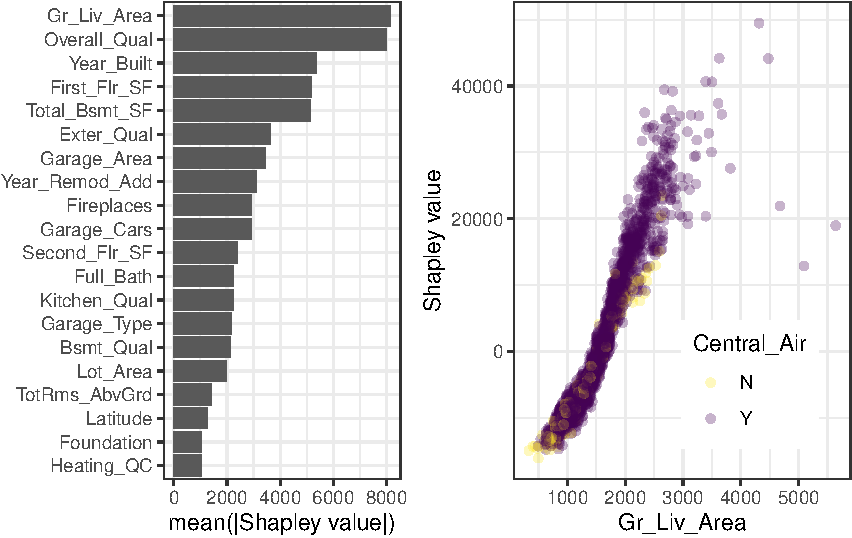
\includegraphics[width=1\linewidth]{greenwell_files/figure-latex/ex-ames-fastshap-autoplot-1} 

}

\caption[Global summary plots of the Ames housing random forest model]{Global summary plots of the Ames housing random forest model. Left: Shapley-based variable importance plot. Right: Shapley-based dependence of predicted sale price on above ground square footage.}\label{fig:ex-ames-fastshap-autoplot}
\end{figure}
\end{Schunk}

\subsubsection{Example: Interfacing with \pkg{shap} via reticulate}

While the \pkg{shapper} package provides a convenient (albeit currently
limited) interface to Python's \textbackslash pkg\{shap package, we're
going to use this example to illustrate how to interface directly with
\pkg{shap} through \pkg{reticulate}.

For illustration, we'll compute feature contributions from a
\dfn{multivariate adaptive regression splines} (MARS) model
\citep{friedman-1991-mars} applied to the well-known Boston housing data
\citep{harrison-1978-hedonic}. MARS models can be fit using the
\CRANpkg{earth} \citep{R-earth} and we'll use the corrected version of
the Boston housing data available in the \CRANpkg{pdp} package
\cite{R-pdp}; see \code{?pdp::boston} for column descriptions and the
original source.

To start, we'll load the data and fit a third degree MARS model (i.e.,
allowing for up to three-way interaction effects) using 5-fold
cross-validation for pruning:

\begin{Schunk}
\begin{Sinput}
library(earth)

# Load the Boston housing data
boston <- pdp::boston
boston$chas <- as.integer(boston$chas) - 1  # coerce to 0/1
X <- subset(boston, select = -cmedv)  # feature columns only

# Fit a third degree MARS model using 5-fold cross-validation
(boston.mars <- earth(cmedv ~ ., data = boston, degree = 3, pmethod = "cv",
                      nfold = 5, ncross = 10))
\end{Sinput}
\begin{Soutput}
#> Selected 17 of 28 terms, and 11 of 15 predictors (pmethod="cv")
#> Termination condition: Reached nk 31
#> Importance: rm, lstat, ptratio, tax, dis, nox, b, crim, age, lon, chas, ...
#> Number of terms at each degree of interaction: 1 7 8 1
#> GRSq 0.9076423  RSq 0.9216937  mean.oof.RSq 0.8038903 (sd 0.11)
#> 
#> pmethod="backward" would have selected:
#>     23 terms 12 preds,  GRSq 0.9121471  RSq 0.9302413  mean.oof.RSq 0.7993457
\end{Soutput}
\end{Schunk}

The fitted model obtained a generalized \(R^2\) (\code{GRSq}) of
\texttt{0.908}. Next, we'll compute feature contributions for each row
in the training set using the KernelSHAP algorithm with \(R = 100\)
repetitions. Before proceeding, we need to define a special prediction
wrapper that will work with the \pkg{shap} package. In this case, it's
about as simple as it gets. In particular, when interfacing with
\pkg{shap}, the prediction wrapper needs to be a function of
\code{newdata} only, which means the fitted model object (in this case,
\code{boston.mars}) needs to be supplied directly to the call to
\code{predict()} inside the function. Further, the output from the
prediction wrapper need to return a data frame or matrix (i.e., it needs
to have a row and column dimension). Fortunately, \pkg{earth}'s predict
method already returns the predictions in a matrix, so we don't need to
do anything further here.

\begin{Schunk}
\begin{Sinput}
# Prediction wrapper for use with `shap$KernelExplainer()`
pfun.shap <- function(newdata) {  # Note: only a function of newdata!
  predict(boston.mars, newdata = newdata)  
}  # returns an `nrow(newdata)` x 1 matrix of predictions
\end{Sinput}
\end{Schunk}

Next, we'll use \pkg{reticulate} to interface directly with the Python
\pkg{shap}
module\^{}\footnote{You need to make sure that you have Python installed, as well as the \pkg{shap} package. If you need help setting up \pkg{reticulate}, see the vignette \code{vignette("calling\_python", package = "reticulate")}.}
and use it to run KernelSHAP (Section \ref{sec:KernelSHAP}) on our
fitted MARS model. We'll request SHAP values for the entire training
set. For comparison, we'll time the expression using
\code{system.time()}. For nicer printing, we convert the results to a
tibble using the \CRANpkg{tibble} package \citep{R-tibble}. (Note that,
as indicated, the following expression will take a few minutes to run.)

\begin{Schunk}
\begin{Sinput}
library(reticulate)

# Import {shap} and run KernelSHAP algorithm with 100 repetitions
shap <- import("shap")
explainer <- shap$KernelExplainer(pfun.shap, data = X)  # initialize explainer
system.time({  # time KernelSHAP
  ex.ks <- explainer$shap_values(X, nsamples = 100L)
})
ex.ks <- ex.ks[[1L]]  # results returned as a list
colnames(ex.ks) <- colnames(X)  # add column names
(ex.ks <- tibble::as_tibble(ex.ks))  # for nicer printing
\end{Sinput}
\end{Schunk}

\begin{verbatim}
#>    user  system elapsed 
#> 558.527  28.887 343.433
\end{verbatim}

\begin{Schunk}
\begin{Soutput}
#> # A tibble: 506 x 15
#>       lon    lat   crim    zn indus  chas   nox    rm    age    dis   rad    tax
#>     <dbl>  <dbl>  <dbl> <dbl> <dbl> <dbl> <dbl> <dbl>  <dbl>  <dbl> <dbl>  <dbl>
#>  1 -0.637  0      0         0 0         0 0      0     0      0     0     -1.18 
#>  2 -0.711  0     -0.191     0 0         0 1.20  -1.43 -0.350 -0.874 0      0.616
#>  3  0      0      0         0 0         0 0      4.71  0      0     0      0    
#>  4  0      0      0         0 0         0 0.517  2.17  0.722  0     0      0    
#>  5  0.930  0      0         0 0.581     0 0.274  3.92  0.277  0     0.463  0.196
#>  6  1.51  -0.350  0         0 0         0 1.09  -1.09  0     -1.43  0      0    
#>  7  0     -0.155 -0.184     0 0         0 0.756 -2.15  0.309 -1.36  0      0    
#>  8  0     -0.440 -0.255     0 0         0 1.04  -1.82 -0.925 -1.57  0      0    
#>  9  0.635 -0.502  0         0 0         0 1.13  -3.03 -1.09  -2.03  0      0    
#> 10  0.860 -0.811  0         0 0         0 0.671 -2.18  0     -2.36  0      0    
#> # ... with 496 more rows, and 3 more variables: ptratio <dbl>, b <dbl>,
#> #   lstat <dbl>
\end{Soutput}
\end{Schunk}

To get an appreciation for the speed of \pkg{fastshap}'s implementation
of SampleSHAP, let's use \code{fastshap::explain()} to compute
SampleSHAP feature contributions for the entire training set using 100
Monte Carlo repetitions. The results are displayed in Figure
\ref{fig:ex-boston-mars-SampleSHAP}, which shows the Shapley-based
dependence of median home value (\code{cmedv}) on percentage of lower
status of the population (\code{lstat}) using 100 Monte-Carlo
repetitions from KernelSHAP (left) and SampleSHAP (right). The results
are nearly the same. We drew lines at the knot locations MARS used to
build piecewise linear terms with the \code{lstat} predictor (you can
see the know locations for each predictor using
\code{coef(boston.mars)}). Notice how the relationship between the
Shapley contribution to \(\widehat{\mathtt{cmedv}}\) and \code{lstat} is
relatively linear in between each knot location. In this case, the
contribution of \code{lstat} to \(\widehat{\mathtt{cmedv}}\) is
relatively monotonically decreasing, and flattens out after around
\code{lstat = 22.11}.

\begin{Schunk}
\begin{Sinput}
pfun.fastshap <- function(object, newdata) {
  predict(object, newdata = newdata)[, 1L, drop = TRUE]
}  # `fastshap::explain()` requires an atomic vector of predictions
set.seed(1503)  # for reproducibility
system.time({
  ex.ss <- fastshap::explain(boston.mars, X = X, pred_wrapper = pfun.fastshap,
                             nsim = 100)
})
\end{Sinput}
\begin{Soutput}
#>    user  system elapsed 
#>  14.039   0.559  14.796
\end{Soutput}
\begin{Sinput}
# Plot results
par(mfrow = c(1, 2), las = 1)
plot(X$lstat, ex.ks$lstat, col = adjustcolor(2, alpha.f = 0.6),
     xlab = "lstat", ylab = "KernelSHAP")
abline(v = c(0.713, 6.12, 22.11), lty = 2)
plot(X$lstat, ex.ss$lstat, col = adjustcolor(4, alpha.f = 0.6),
     xlab = "lstat", ylab = "SampleSHAP")
abline(v = c(0.713, 6.12, 22.11), lty = 2)
\end{Sinput}
\begin{figure}[!htb]

{\centering 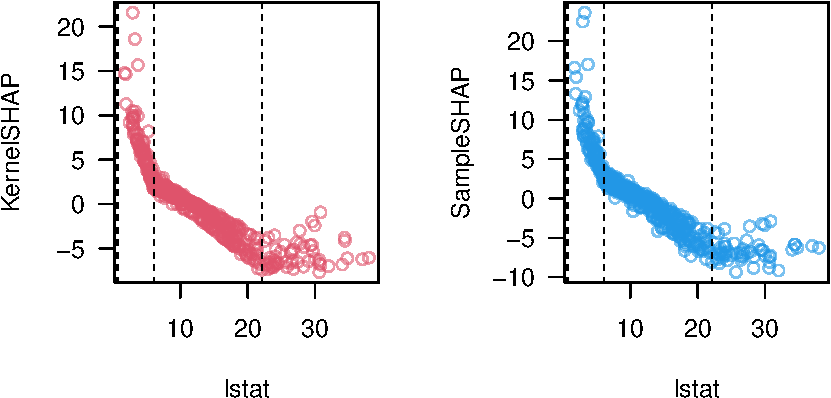
\includegraphics[width=1\linewidth]{greenwell_files/figure-latex/ex-boston-mars-SampleSHAP-1} 

}

\caption[Shapley-based dependence of percentage of lower status of the population (\code{lstat}) on median home value (\code{cmedv}) using 100 Monte-Carlo repetitions from KernelSHAP (left) and SampleSHAP (right)]{Shapley-based dependence of percentage of lower status of the population (\code{lstat}) on median home value (\code{cmedv}) using 100 Monte-Carlo repetitions from KernelSHAP (left) and SampleSHAP (right).}\label{fig:ex-boston-mars-SampleSHAP}
\end{figure}
\end{Schunk}

\subsection{A simple benchmark comparison \label{sec:benchmark}}

This section provides a brief example comparing various implementations
of Shapley values using \href{https://www.kaggle.com/c/titanic}{Kaggle's
Titanic: Machine Learning from Disaster competition}. While the true
focus of the competition is to use machine learning to create a model
that predicts which passengers survived the Titanic shipwreck, we'll
focus on explaining predictions from a simple logistic regression model.

To start, we'll load the data, which are conveniently available in the
\CRANpkg{titanic} package \citep{R-titanic}, and do a little bit of
cleaning.

\begin{Schunk}
\begin{Sinput}
# Read in the data and clean it up a bit
titanic <- titanic::titanic_train
features <- c(
  "Survived",  # passenger survival indicator
  "Pclass",    # passenger class
  "Sex",       # gender
  "Age",       # age
  "SibSp",     # number of siblings/spouses aboard
  "Parch",     # number of parents/children aboard
  "Fare",      # passenger fare
  "Embarked"   # port of embarkation
)
titanic <- titanic[, features]
titanic$Survived <- as.factor(titanic$Survived)
titanic <- na.omit(titanic)

# Data frame containing just the features
X <- subset(titanic, select = -Survived)
\end{Sinput}
\end{Schunk}

Next, we'll use the stats::glm() to fit a logistic regression model with
only main effects (i.e., no tw-way interactions, etc.).

\begin{Schunk}
\begin{Sinput}
fit <- glm(Survived ~ ., data = titanic, family = binomial)
\end{Sinput}
\end{Schunk}

Suppose we wanted to explain the predicted survival probability for a
new passenger named Jack
Dawson\footnote{Inspiration for this example was taken from \url{https://modeloriented.github.io/iBreakDown/articles/vignette_iBreakDown_titanic.html.}}:

\begin{Schunk}
\begin{Sinput}
jack.dawson <- data.frame(
  Pclass = 3,
  Sex = factor("male", levels = c("female", "male")),
  Age = 20,
  SibSp = 0,
  Parch = 0,
  Fare = 15,  # lower end of third-class ticket prices; technically, Jack won his ticket
  Embarked = factor("S", levels = c("", "C", "Q", "S"))
)
\end{Sinput}
\end{Schunk}

Our logistic regression model predicts that Jack's log-odds of survival
is

\begin{Schunk}
\begin{Sinput}
predict(fit, newdata = jack.dawson)
\end{Sinput}
\begin{Soutput}
#>         1 
#> -1.845561
\end{Soutput}
\end{Schunk}

Yikes, that's equivalent to estimated 13.64\% predicted probability of
survival! With a baseline (i.e., average) survival rate of 40.62\%, can
we explain why the model predicts Jack to be much lower?
Enter\ldots Shapley values.

There is a growing number of R packages that provide Shapley
explanations, the two most popular arguably being \pkg{iml} and
\pkg{iBreakDown}. In this example, we'll compare those with
\pkg{fastshap}.

To start, we need to define a few things (prediction wrapper, as well as
both \pkg{iml}- and \pkg{iBreakDown}-related helpers).

\begin{Schunk}
\begin{Sinput}
# Prediction wrapper to compute predicted probability of survive
pfun <- function(object, newdata) {
  predict(object, newdata = newdata)
}

# DALEX-based helper for iBreakDown
explainer <- DALEX::explain(fit, data = X, y = titanic$Survived,                                             predict_function = pfun, verbose = FALSE)

# Helper for iml
predictor <- iml::Predictor$new(fit, data = titanic, y = "Survived",
                                predict.fun = pfun)
\end{Sinput}
\end{Schunk}

Next, we call each implementation's Shapley-related function to compute
explanations for Jack's prediction using 100 Monte Carlo repetitions.

\begin{Schunk}
\begin{Sinput}
# Compute explanations
set.seed(1039)  # for reproducibility
ex1 <- iBreakDown::shap(explainer, B = 100, new_observation = jack.dawson)
ex2 <- iml::Shapley$new(predictor, x.interest = jack.dawson, sample.size = 100)
ex3 <- fastshap::explain(fit, X = X, pred_wrapper = pfun, nsim = 100,
                         newdata = jack.dawson)
\end{Sinput}
\end{Schunk}

Finally, we plot the resulting explanations. Note that both
\pkg{fastshap} and \pkg{iBreakDown} plot the feature contributions in
the original order, whereas \pkg{iml} plots them in descending order.

\begin{Schunk}
\begin{Sinput}
# Plot results (see Figure XYZ)
p3 <- plot(ex1) + ggtitle("iBreakDown")
p2 <- plot(ex2) + ggtitle("iml")
p1 <- autoplot(ex3, type = "contribution") + ggtitle("fastshap")
gridExtra::grid.arrange(p1, p2, p3, nrow = 1)
\end{Sinput}
\begin{figure}[!htb]

{\centering 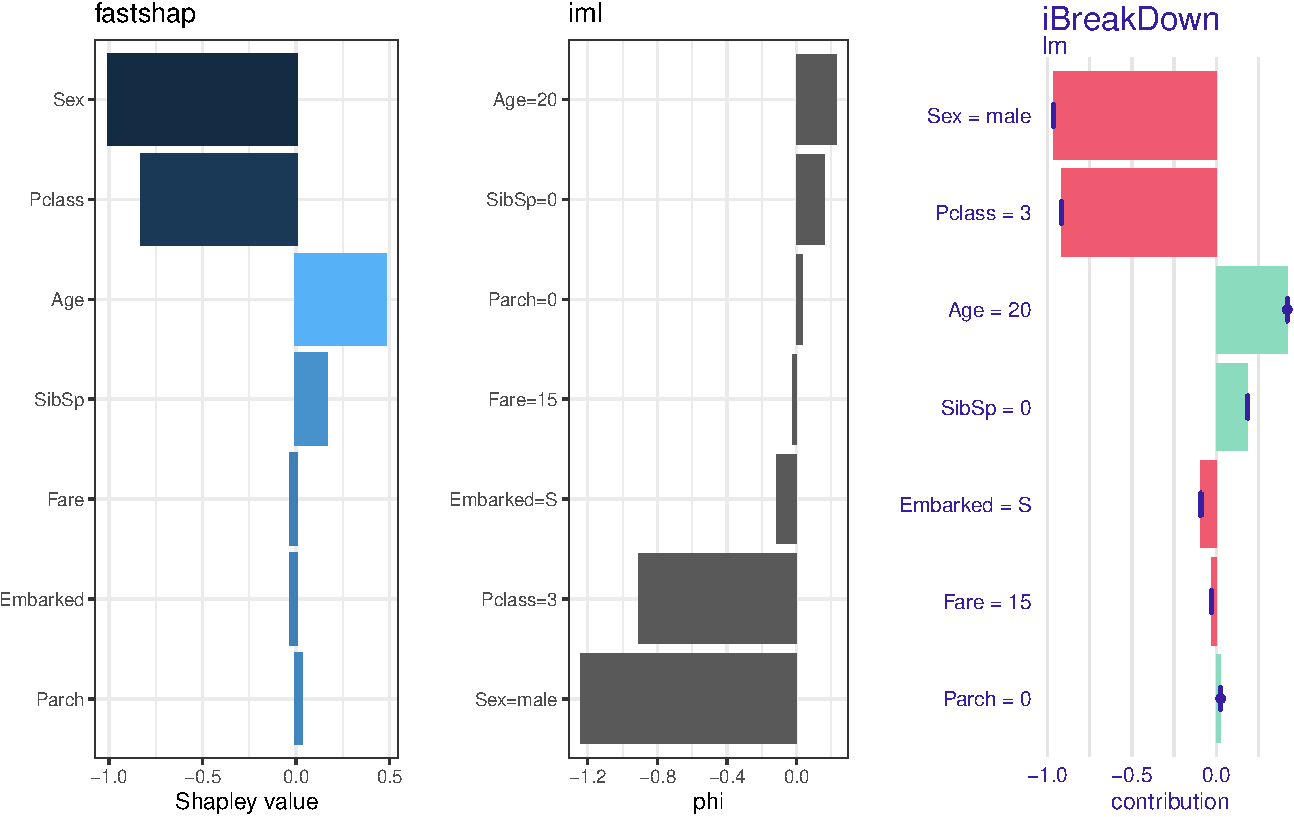
\includegraphics[width=1\linewidth]{greenwell_files/figure-latex/titanic-jack-explanations-plot-1} 

}

\caption[Feature contributions for the tianic example using three different implementations of SampleSHAP]{Feature contributions for the tianic example using three different implementations of SampleSHAP.}\label{fig:titanic-jack-explanations-plot}
\end{figure}
\end{Schunk}

Each package comes loaded with it's own bells and whistles (e.g.,
\pkg{iml} and \pkg{iBreakDown} have particularly fantastic
visualizations). The main selling point of \pkg{fastshap} is speed! For
example, all three packages (in fact, all general and practical
implementations of Shapley values) use Algorithm \ref{alg:SampleSHAP}
which requires a large number of Monte Carlo repetitions to achieve
accurate results. Below is a simple benchmark looking at the estimated
time (in seconds) to explain Jack's prediction as a function of the
number of Monte Carlo repetitions for each implementation. (Note that
this comparison does not make use of \pkg{fastshap}'s feature-wise
parallelization.)

\begin{Schunk}
\begin{Sinput}
# Number of Monte Carlo reps for each simulation
nsims <- c(1, 5, 10, 25, 50, 75, seq(from = 100, to = 1000, by = 100))

# Initialize vectors to store timings
times1 <- times2 <- times3 <- numeric(length(nsims))

# Run simulation
set.seed(904)  # for reproducibility
for (i in seq_along(nsims)) {  # iBreakDown
  message("nsim = ", nsims[i], "...")
  times1[i] <- system.time({
    iBreakDown::shap(explainer, B = nsims[i], new_observation = jack.dawson)
  })["elapsed"]
  times2[i] <- system.time({  # iml
    iml::Shapley$new(predictor, x.interest = jack.dawson, 
                     sample.size = nsims[i])
  })["elapsed"]
  times3[i] <- system.time({  # fastshap
    fastshap::explain(fit, X = X, newdata = jack.dawson, pred_wrapper = pfun, 
                      nsim = nsims[i])
  })["elapsed"]
}

# Plot results
palette("Okabe-Ito")  # colorblind friendly palette 
plot(nsims, times1, type = "b", xlab = "Number of Monte Carlo repetitions",
     ylab = "Time (in seconds)", las = 1, pch = 19, 
     xlim = c(0, max(nsims)), ylim = c(0, max(times1, times2, times3)))
lines(nsims, times2, type = "b", pch = 19, col = 2)
lines(nsims, times3, type = "b", pch = 19, col = 3)
legend("topleft",
       legend = c("iBreakDown", "iml", "fastshap"),
       lty = 1, pch = 19, col = 1:3, inset = 0.02)
\end{Sinput}
\begin{figure}[!htb]

{\centering 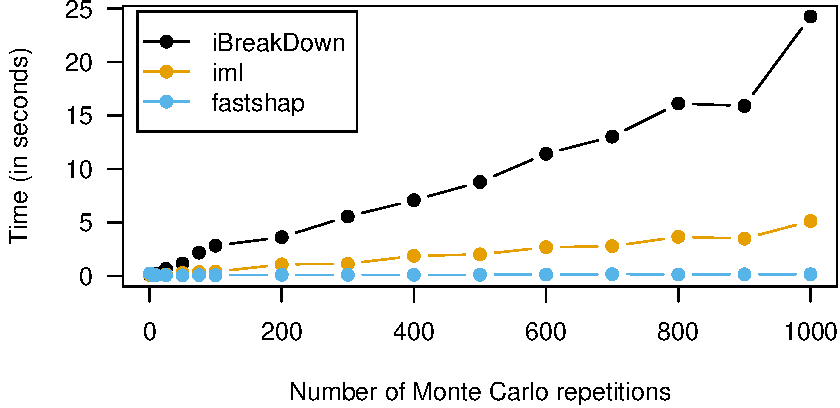
\includegraphics[width=1\linewidth]{greenwell_files/figure-latex/titanic-benchmark-1} 

}

\caption[Quick benchmark between three different implementations of SampleSHAP for explaining Jack's unfortunate prediction]{Quick benchmark between three different implementations of SampleSHAP for explaining Jack's unfortunate prediction.}\label{fig:titanic-benchmark}
\end{figure}
\begin{Sinput}
palette("default")  # switch back to R's default color palette
\end{Sinput}
\end{Schunk}

The message to be taken from Figure \ref{fig:titanic-benchmark} is that
\pkg{fastshap} scales incredibly well with \(N\) or \(R\), as long as
the corresponding \code{predict()} method does.

Oh, and \pkg{fastshap} can produce instant (and exact) Shapley
contributions for this example using LinearSHAP (Section
\ref{sec:LinearSHAP}):

\begin{Schunk}
\begin{Sinput}
fastshap::explain(fit, newdata = jack.dawson, exact = TRUE)  # ExactSHAP
\end{Sinput}
\begin{Soutput}
#> # A tibble: 1 x 7
#>   Pclass    Sex   Age SibSp  Parch    Fare Embarked
#>    <dbl>  <dbl> <dbl> <dbl>  <dbl>   <dbl>    <dbl>
#> 1 -0.915 -0.964 0.420 0.186 0.0260 -0.0282  -0.0919
\end{Soutput}
\begin{Sinput}
fastshap::explain(fit, X = X, pred_wrapper = pfun, nsim = 10000,
                  newdata = jack.dawson)  # SampleSHAP
\end{Sinput}
\begin{Soutput}
#> # A tibble: 1 x 7
#>   Pclass    Sex   Age SibSp  Parch    Fare Embarked
#>    <dbl>  <dbl> <dbl> <dbl>  <dbl>   <dbl>    <dbl>
#> 1 -0.929 -0.977 0.422 0.185 0.0257 -0.0290  -0.0865
\end{Soutput}
\begin{Sinput}
predict(fit, newdata = jack.dawson, type = "terms")  # ExactSHAP (base R)
\end{Sinput}
\begin{Soutput}
#>       Pclass        Sex       Age     SibSp      Parch       Fare    Embarked
#> 1 -0.9153946 -0.9644851 0.4204564 0.1861824 0.02599872 -0.0281944 -0.09194646
#> attr(,"constant")
#> [1] -0.4781785
\end{Soutput}
\end{Schunk}

\hypertarget{summary}{%
\subsection{Summary}\label{summary}}

This file is only a basic article template. For full details of
\emph{The R Journal} style and information on how to prepare your
article for submission, see the
\href{https://journal.r-project.org/share/author-guide.pdf}{Instructions
for Authors}.

\bibliography{greenwell}


\address{%
Brandon M. Greenwell\\
University of Cincinnati\\%
2925 Campus Green Dr\\ Cincinnati, OH 45221\\ United States of
America\\ ORCiD---\href{https://orcid.org/0000-0002-8120-0084}{0000-0002-8120-0084}\\
%
%
%
\\\href{mailto:greenwell.brandon@gmail.com}{\nolinkurl{greenwell.brandon@gmail.com}}
}

\address{%
Christoph Molnar\\
TBD\\%
TBD\\ TBD\\ TBD\\
%
%
%
\\TBD
}
